\section{Задание №2}

\begin{enumerate}
        \item Построить датчик сингулярного распределения, имеющий в качестве функции распределения канторову лестницу. С помощью критерия Колмогорова убедиться в корректности работы датчика.
        \item Для канторовых случайных величин проверить свойство симметричности относительно $\frac12$ ($X$ и $(1 - X)$ распределены одинаково) и самоподобия относительно деления на $3$ (условное распределение $Y$ при условии $Y\in[0,\,\frac13]$ совпадает с распределением $\frac{Y}{3}$) с помощью критерия Смирнова.
        \item Вычислить значение математического ожидания и дисперсии с эмпирическими для разного объема выборок. Проиллюстрировать сходимость.
\end{enumerate}


\subsection{Построение датчика <<канторовой>> случайной величины}
\begin{definition}
        Пусть дано вероятностное пространство $(\R,\, \mathcal{F},\,\p)$, и на нем определена случайная величина $\xi$ с распределением $\p_\xi$. Тогда \textit{функцией распределения} случайной величины $X$ называется функция $F_\xi:\,\R\to[0,\,1]$, задаваемая формулой:
        $$
                F_\xi(x) = \p(\xi\leqslant x) \equiv \p_\xi(\,(-\infty,\,x]\,). 
        $$
\end{definition}

\begin{definition}
        Функция распределения некоторой случайной величины называется \textit{сингулярной}, если она непрерывна и ее множество точек роста имеет нулевую меру Лебега.
\end{definition}

\begin{definition}
        Из единичного отрезка $C_0 = [0,\,1]$ удалим интервал $\left(\frac13,\,\frac23\right)$. Оставшееся множество обозначим за $C_1$. Множество $C_1 = \left[0,\,\frac13\right]\cup\left[\frac23,\,1\right]$ состоит из двух отрезков; удалим теперь из каждого отрезка его среднюю часть, и оставшееся множество обозначим за $C_2$. Повторив данную процедуру, то есть удаляя средние трети у всех четырех отрезков, получим $C_3$. Дальше таким же образом получаем последовательность замкнутых множеств $C_0 \supset C_1 \supset C_2 \supset \ldots \supset C_i \supset \ldots$. Пересечение
        $$
                C = \bigcap_{i=0}^{\infty} C_i
        $$
        называется \textit{канторовым множеством}.
\end{definition}

\begin{remark}
        Канторово множество так же можно определить как множество всех чисел от нуля до единицы, которые можно представить в троичной записи при помощи только нулей и двоек. То есть
        $$
                C = \{\,0,\alpha_1\,\alpha_2\,\ldots\,\alpha_i\,\ldots\,_3\:|\:\alpha_i=0,\,2\,\}.
        $$
\end{remark}

\begin{assertion}
        Канторово множество имеет нулевую меру Лебега. \cite{shiryaev}
\end{assertion}

\begin{definition}
        Рассмотрим функцию $K(x)$ такую, что в точках $0$ и $1$ значение функции принимается равным соответственно $0$ и $1$.
        Далее интервал $(0,\,1)$ разбивается на три равные части $\left(0,\,\frac {1}{3}\right)$, $\left(\frac{1}{3},\,\frac {2}{3}\right)$ и $\left(\frac{2}{3},\,1\right)$.
        На среднем сегменте полагаем $K(x)=\frac{1}{2}$.
        Оставшиеся два сегмента снова разбиваются на три равные части каждый, и на средних сегментах $K(x)$ полагается равной $\frac{1}{4}$ и $\frac{3}{4}$.
        Каждый из оставшихся сегментов снова делится на три части, и на внутренних сегментах $K(x)$ определяется как постоянная, равная среднему арифметическому между соседними, уже определенными значениями $K(x)$.
        На остальных точках единичного отрезка определяется по непрерывности.
        Полученная функция называется \textit{канторовой лестницей}. 
\end{definition}

\begin{remark}
        Из определения канторовой лестницы~$K(x)$ следует, что она действует на точки из канторова множества $C$ по следующему правилу:
        $$
                K(0,\alpha_1\,\alpha_2\,\ldots\,\alpha_i\,\ldots\,_3) =
                0,\frac{\alpha_1}2\,\frac{\alpha_2}2\,\ldots\,\frac{\alpha_i}2\,\ldots\,_2.
        $$
\end{remark}

Теперь рассмотрим случайную величину 
$$
        Y =
        0, \xi_1\,\xi_2\ldots\xi_k\,\ldots\,_2 =
        \sum_{k=1}^{\infty}\frac{\xi_k}{2^k},
        \quad
        \mbox{где $\xi_k \sim\mbox{Bern}\left(\frac12\right)$}.
$$
Такая случайная величина имеет равномерное распределение на откезке $[0,1]$, так как мы равновероятным образом выбираем знаки разложения числа~$\xi_k$ в двоичном представлении. Теперь рассмотрим искомую случайную величину~$X$, имеющую в качестве функции распределения~$F_X(x)$ канторову лестницу~$K(x)$. Образ каждой случайной величины $Y$ для такой функции будет равен
$$
        K^{-1}(Y) = \sum_{k=1}^{\infty}\frac{2\xi_k}{3^k}.
$$
Эта точка лежит в канторовом множестве.

\begin{theorem}
\label{th:th2-1}
        Пусть некоторая функция распределения $F$ имеет обратную $F^{-1}$. Тогда функцией распределения случайной величины
        $$
                \eta = F^{-1}(\xi),
        $$
        где $\xi$~--- равномерно распределенная на отрезке $[0,\,1]$ случайная величина, является $F$.
\end{theorem}
\begin{proof}
        Найдем функцию распределения случайной величины $\eta$:
        $$
                F_\eta(x) =
                \p(\eta \leqslant x) =
                \p(F^{-1}(\xi) \leqslant x) =
                \p(\xi \leqslant F(x)) =
                F(x).
        $$
        Таким образом, теорема доказана.
\end{proof}

Из теоремы вытекает, что при помощи построенного ранее (см. раздел~\ref{task_01}) генератора схемы Бернулли мы можем смоделировать случайную величину $X$, принимающую с вероятностью $1$ значения из канторова множества~C и имеющую канторову лестницу~$K(x)$ в качестве функции распределения~$F_X(x)$, следующим образом:
$$
        X = \sum_{k = 1}^{\infty}\frac{2\xi_k}{3^k},
        \quad
        \mbox{где $\xi_k\sim\mbox{Bern}\left(\frac12\right)$.}
$$

В программной реализации будем рассматривать частичные суммы. Для этого этого введем погрешность $\varepsilon$ и найдем такое число $n$, при котором частичная сумма будет отличаться от бесконечной не более, чем на заданную погрешность.
$$
        \sum_{k=n}^{\infty} \frac{2\xi_k}{3^k} \leqslant 2\sum_{k=n}^{\infty}\frac{1}{3^k} = \frac{1}{3^{n-1}} \leqslant \varepsilon,
$$
$$
        \Downarrow
$$
$$
        n \geqslant 1 - \left\lceil\,\log_3 \varepsilon\,\right\rceil \; \forall \varepsilon < 1.
$$
\begin{remark}
        Из выведенной формулы также видно, что для столь малой погрешности как $\varepsilon = 10^{-9}$ достаточно использовать всего $n = 20$ первых членов ряда.
\end{remark}


\subsection{Проверка корректности работы датчика}
\begin{definition}
        Пусть задана выборка $\xi = (\xi_1,\,\xi_2,\,\ldots,\,\xi_n)$, где $\xi_i \in \Xi, i = \overline{1,\,n}$. \textit{Эмперической (выборочной) функцией распределения}, построенной на этой выборке, называется функция $F_n(x)$, равная доле таких значений $\xi_i$, что $\xi_i < x$. Или другими словами
$$
        F_n(x) = \frac{1}{n}
        \sum_{i = 1}^n \mathbb{I}_{(-\infty,\,x)}(\xi_i),
        \quad
        \mbox{где }
        \mathbb{I}_{(-\infty,\,x)}(\xi_i)
        =
        \begin{cases}
                1, & \mbox{при } \xi_i < x, \\
                0, & \mbox{иначе.}
        \end{cases}
$$
\end{definition}
\begin{definition}
        Пусть в некотором эксперименте доступна наблюдению случайная величина $\xi$, распределение которой $\p$ полностью или частично неизвестно. Тогда любое утверждение относительно $\p$ называется \textit{статистической гипотезой} $H$.
\end{definition}
\begin{theorem}[Критерий согласия Колмогорова]
        Обозначим нулевую гипотезу $H_0$ как гипотезу о том, что выборка подчиняется распределению $F(\xi) \in C^1(\Xi)$. Введем статистику критерия
$$
        D_n = \sup\limits_{x}|F_n(x) - F(x)|.
$$
        Тогда если гипотеза $H_0$ верна, то $\sqrt{n}D_n$ с ростом $n$ сходится по распределению к случайной величине $K$ с функцией распределения Колмгорова
$$
        F_K(x) = 1 + 2\sum_{i = 1}^{+\infty} (-1)^k e^{-2k^2x^2}.
$$
\end{theorem}
\begin{remark}
        Гипотеза $H_0$ отвергается, если при большом объеме выборки $n$ статистика $\sqrt{n}D_n$ превышает квантиль распределения $K_\alpha$, заданного \textit{уровня значимости} $\alpha$, и принимается в противном случае. Здесь $K_\alpha = F_K^{-1}(1 - \alpha)$.
\end{remark}

В рамках реализации подсчет $K_\alpha$ в явном виде весьма трудоемкая задача. Поэтому мы будем расчитывать \textit{p-значение} для нашей статистики $p_{value} = 1 - F_K(\sqrt{n}D_n)$. Если p-значение оказалось ниже или равно установленному уровню значимости $\alpha$, то наша гипотеза отвергается и применяется альтернативная.

\begin{table}[h]
\begin{center}
\begin{tabular}{|c|c|c|c|}
\hline
Число испытаний &
Размер выборки  &
Уровень значимости &
Частота принятия гипотезы
\\
\hline
$10^3$
&
$10^3$
&
$0,05$
&
$0,958$
\\
\hline
$10^4$
&
$10^3$
&
$0,05$
&
$0,9536$
\\
\hline
$10^3$
&
$10^4$
&
$0,05$
&
$0,959$
\\
\hline
$10^3$
&
$10^3$
&
$0,1$
&
$0,907$
\\
\hline
\end{tabular}
\end{center}
\caption{Частота принятия гипотезы $H_0$ о том, что построенный датчик случайной величины имеет канторову лестницу в качестве функции распределения. Из таблицы видно, что вероятность отклонить гипотезу не превышает допустимый уровень значимости.}
\end{table}


\subsection{Симметричность <<канторовой>> случайной величины относительно~\nicefrac{1}{2}}

\begin{assertion}[Свойство симметричности относительно \nicefrac{1}{2}]
        Пусть $X$ --- случайная величина, с канторовой лестницей в качестве функции распределения. Тогда верно
$$
        F_X(x) = F_{1-X}(x).
$$
\end{assertion}
\begin{proof}
        Как мы помним из построения датчика <<канторовой>> случайной величины, она представима в виде:
$$
        X = 2 \sum_{k=1}^\infty\frac{\xi_k}{3^k},
        \quad
        \mbox{где } \xi_k \sim \mbox{Bern}\left(\nicefrac{1}{2}\right), k = \overline{1, n}.
$$
        Тогда
$$
        1 - X
        =
        1 - 2 \sum_{k=1}^\infty\frac{\xi_k}{3^k}
        =
        2 \sum_{k=1}^\infty\frac{1}{3^k} - 2 \sum_{k=1}^\infty\frac{\xi_k}{3^k}
        =
        2 \sum_{k=1}^\infty\frac{1 - \xi_k}{3^k}
        =
        2 \sum_{k=1}^\infty\frac{\eta_k}{3^k},
$$ 
        при этом случайная величины $\eta_k = 1 - \xi_k$ также имеют распределение Бернулли с параметром $p = \nicefrac{1}{2}$. Значит, случайные величины $X$ и $1 - X$ имеют одинаковое распределение.

\end{proof}

Теперь эмперическим путем убедимся в выполнении этого свойства. Для этого нам потребуется \textit{критерий Смирнова}. Он используется для проверки гипотезы о принадлежности двух независимых выборок одному и тому же распределению.

\begin{theorem}[Критерий однородности Смирнова]
        Обозначим за нулевую гипотезу $H_0$ гипотезу о том, что две исследуемые выборки объемами $n$ и $m$ с эмперическими функциями распределения $F_n(x)$ и $F_m(x)$ соответственно распределениы по одному закону. Введем статистику критерия
$$
        D_{n,\,m} = \sup\limits_{x}|F_n(x) - F_m(x)|.
$$
Тогда если гипотеза $H_0$ верна, то при увеличении объемов выборок $n$ и $m$ случайная величина $\sqrt{\frac{nm}{n + m}}D_{n,m}$ будет сходиться по распределению к случайной величине $K$ с функцией распределения Колмогорова
$$
       F_K(x) = 1 + 2\sum_{i = 1}^{+\infty} (-1)^k e^{-2k^2x^2}. 
$$
\end{theorem}


\subsection{Самоподобие <<канторовой случайной величины относительно деления на 3}

\begin{assertion}[Свойство самоподобия относительно деления на 3]
        Пусть $X$ --- случайная величина с канторовой лестницей в качестве функции распределения. Тогда верно
$$
        F_{\nicefrac{X}{3}}(x) = F_{X\,|\,X\in[0,\,\nicefrac{1}{3}]}(x).
$$
\end{assertion}
\begin{proof}
        Заметим, что из построения датчика <<канторовой>> случайной величины вытекает, что случайная величина $Y = X\,|\, X \in [0,\,\nicefrac{1}{3}]$ задается в виде
$$
        X = 2 \sum_{k=1}^{\infty}\frac{\xi_k}{3^k},
        \quad
        \mbox{где } \xi_1 = 0,\,\xi_k \sim \mbox{Bern}(\nicefrac{1}{2}), k = \overline{2, n}.
$$
Тогда получается, что
$$
        Y
        =
        2 \sum_{k=2}^\infty\frac{\xi_k}{3^k}
        =
        2 \sum_{k=1}^\infty\frac{\xi_{k+1}}{3^{k+1}}
        =
        \frac{2}{3} \sum_{k=1}^\infty\frac{\xi_k}{3^k}
        =
        \frac{X}{3}.
$$

\end{proof}

Так же проверим получившийся результат при помощи критерия однородности Смирнова.

\begin{table}[h!]
\begin{center}
\begin{tabular}{|c|c|c|c|}
\hline
Число испытаний
&
$10^3$&
$10^3$&
$10^3$
\\
\hline
Размер первой выборки
&
$10^2$&
$10^3$&
$10^3$
\\
\hline
Размер второй выборки
&
$10^3$&
$10^3$&
$10^3$
\\
\hline
Уровень значимости
&
$0,05$&
$0,05$&
$0,01$
\\
\hline
Частота принятия гипотезы
&
$0,956$&
$0,955$&
$0,912$
\\
\hline
\end{tabular}
\end{center}
\caption{Частота принятия гипотезы $H_0$ о том, что случайные величины $X$ и $(1 - X)$ имеют одинаковое распределение.}
\end{table}

\begin{table}[h!]
\begin{center}
\begin{tabular}{|c|c|c|c|}
\hline
Число испытаний
&
$10^3$&
$10^3$&
$10^3$
\\
\hline
Размер первой выборки
&
$10^2$&
$10^3$&
$10^3$
\\
\hline
Размер второй выборки
&
$10^3$&
$10^3$&
$10^3$
\\
\hline
Уровень значимости
&
$0,05$&
$0,05$&
$0,01$
\\
\hline
Частота принятия гипотезы
&
$0,956$&
$0,955$&
$0,915$
\\
\hline
\end{tabular}
\end{center}
\caption{Частота принятия гипотезы $H_0$ о том, что случайные величины $X\,|\,X\in[0,\,\nicefrac{1}{3}]$ и $\nicefrac{X}{3}$ имеют одинаковое распределение.}
\end{table}


\subsection{Математическое ожидание и дисперсия <<канторовой>> случайной величины}

Вычислим значение математического ожидания для построенной случайной величины $X$:
$$
        \E\,X
        =
        \E\sum_{k=1}^{\infty}\frac{2\xi_k}{3^k}
        =
        \sum_{k=1}^{\infty}\frac{2}{3^k}\E\xi_k=
        \sum_{k=1}^\infty \frac{2}{3^k}\cdot\frac12
        =
        \frac{\frac13}{1 - \frac13}
        =
        \frac{1}{2}.
$$
Теперь, помня о независимости случайных величин $\xi_k\;k\in\N$, вычислим значение дисперсии
$$
        \Var\,X
        =
        \Var\sum_{k=1}^{\infty}\frac{2\xi_k}{3^k}
        =
        \sum_{k=1}^{\infty}\left(\frac{2}{3^k}\right)^2\Var\,\xi_k
        =
        \sum_{k=1}^{\infty}\frac{4}{9^k}\cdot\frac14
        =
        \frac{\frac19}{1 - \frac19}
        =
        \frac18.
$$
\begin{remark}
        При подсчете мы использовали известные значения для математического ожидания и дисперсии бернуллиевой случайной величины $\xi\sim\mbox{Bern}(p)$:
        $$
                \E\,\xi = p
                \quad
                \mbox{и}
                \quad
                \Var\,\xi = p(1-p).
        $$
\end{remark}

Для сравнения практического и теоретического результатов построим также графики \textit{выборочного среднего} $\overline{X}$ и \textit{несмещенной выборочной дисперсии} $S^2$, задаваемых формулами:
$$
        \overline{X} = \frac{1}{n}\sum_{i=1}^n X_i
        \quad
        \mbox{и}
        \quad
        S^2 = \frac{1}{n-1}\sum_{i=1}^n(X_i - \overline{X})^2.
$$


\clearpage
\begin{figure}[t]
        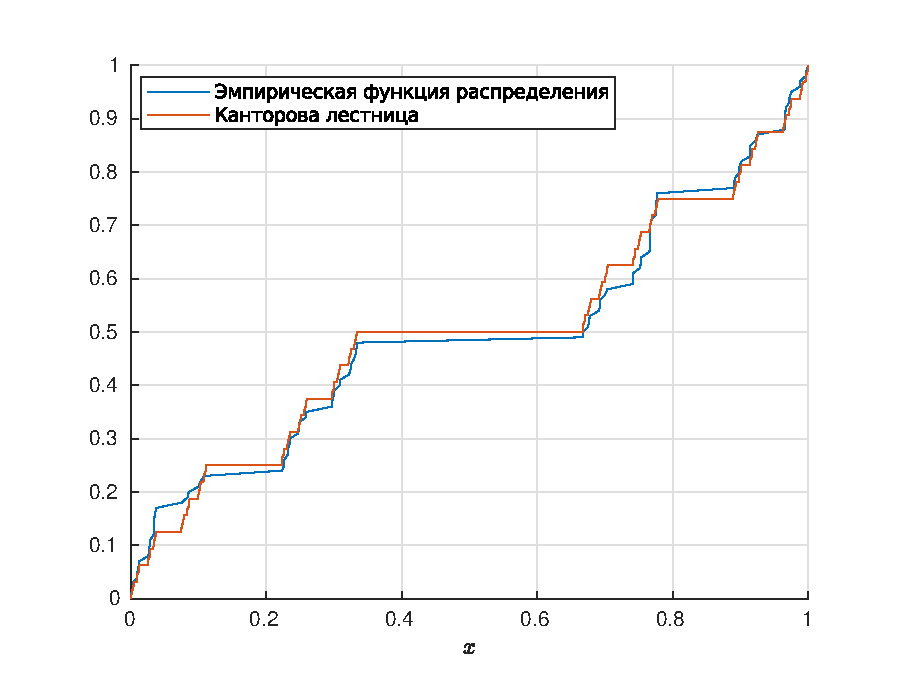
\includegraphics[width=0.5\linewidth]{task_02/cantor-100.eps}
        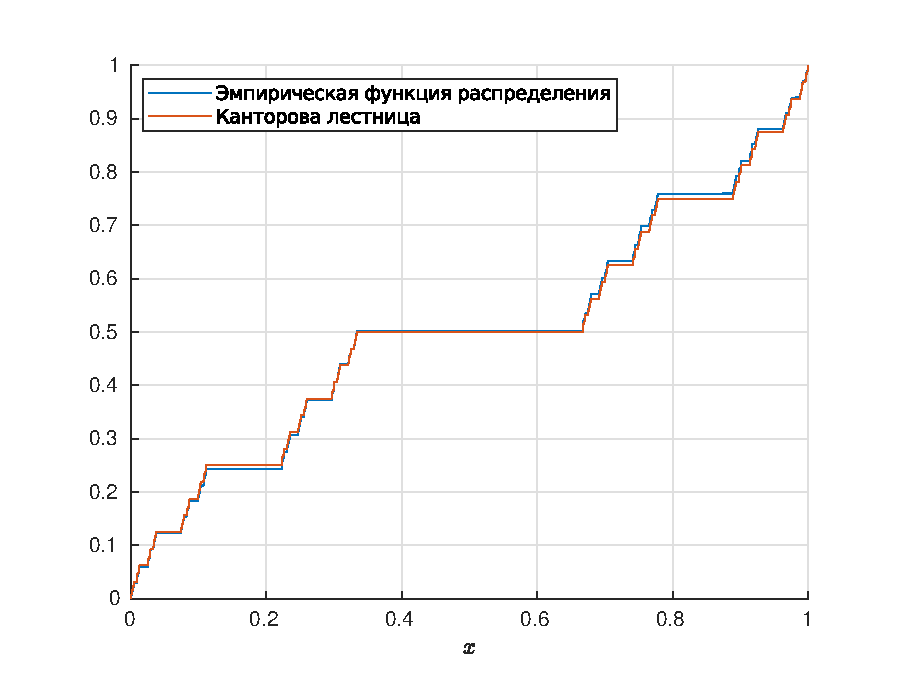
\includegraphics[width=0.5\linewidth]{task_02/cantor-10000.eps}
        \caption{Эмпирическая и теоретическая функции распределения <<канторовой>> случайной величины $X$ при выборке из $100$~испытаний~(слева) и $10^4$~испытаний~(справа).}
\end{figure}
\begin{figure}[b]
        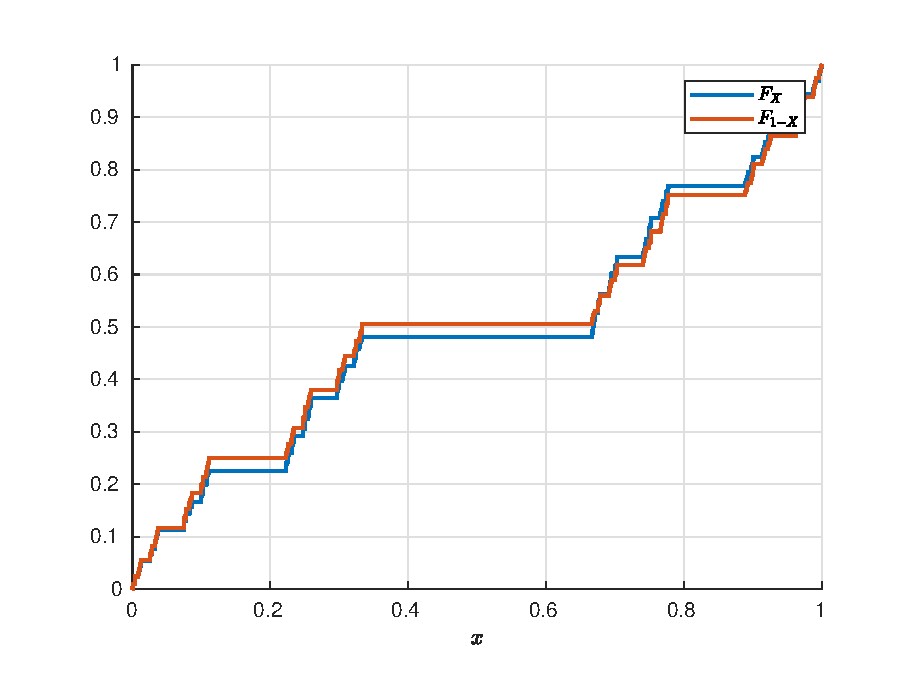
\includegraphics[width=0.5\linewidth]{task_02/sim-1000.eps}
        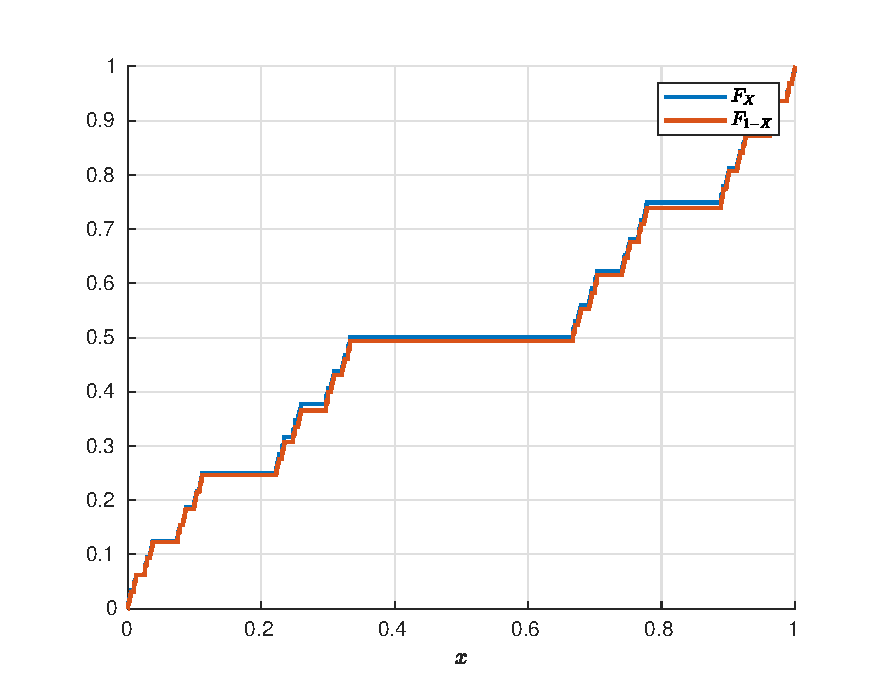
\includegraphics[width=0.5\linewidth]{task_02/sim-10000.eps}
        \caption{График, иллюстрирующий свойство симметричности относительно \nicefrac{1}{2} <<канторовой>> случайной величины. Представлены эмперические функции распределения при объемах выборок $10^3$~(слева) и $10^4$~(справа).}
\end{figure}

\begin{figure}[t]
        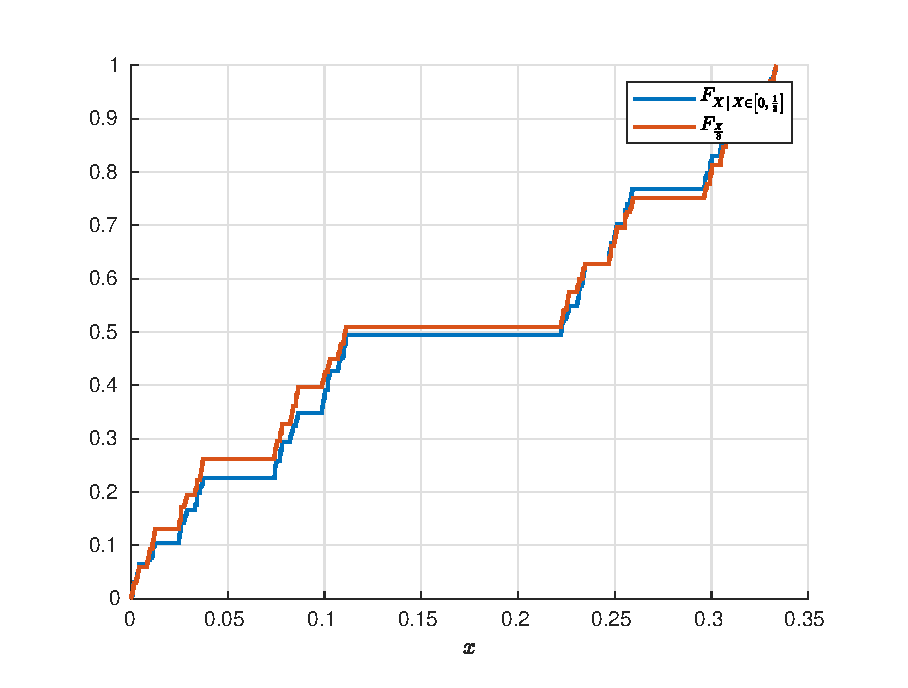
\includegraphics[width=0.5\linewidth]{task_02/sam-1000.eps}
        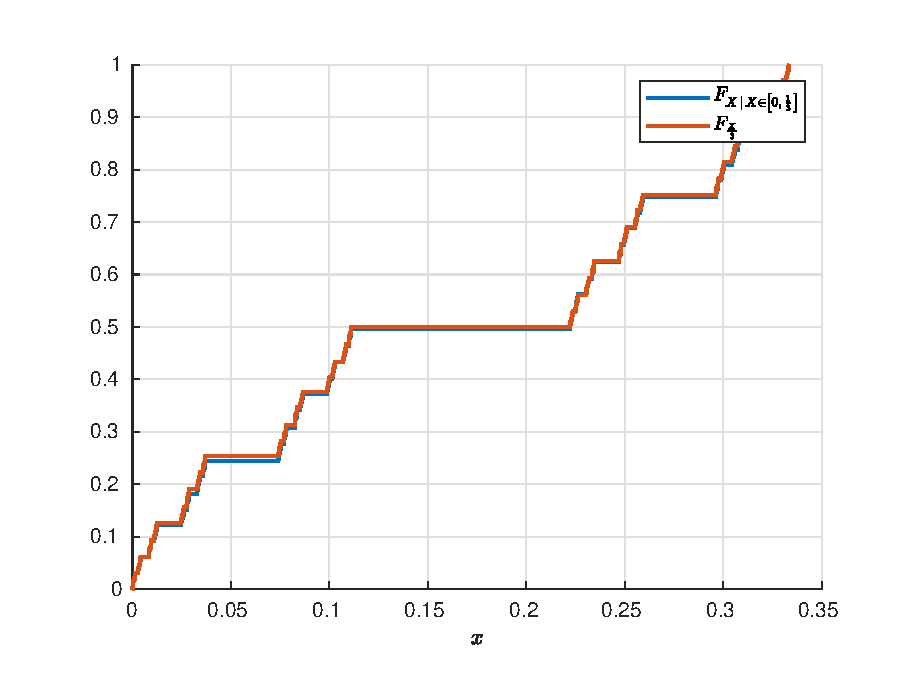
\includegraphics[width=0.5\linewidth]{task_02/sam-10000.eps}
        \caption{График, иллюстрирующий свойство самоподобия относительно деления на 3 <<канторовой>> случайной величины. Представлены эмперические функции распределения при объемах выборок $10^3$~(слева) и $10^4$~(справа).}
\end{figure}

\begin{figure}[b]
        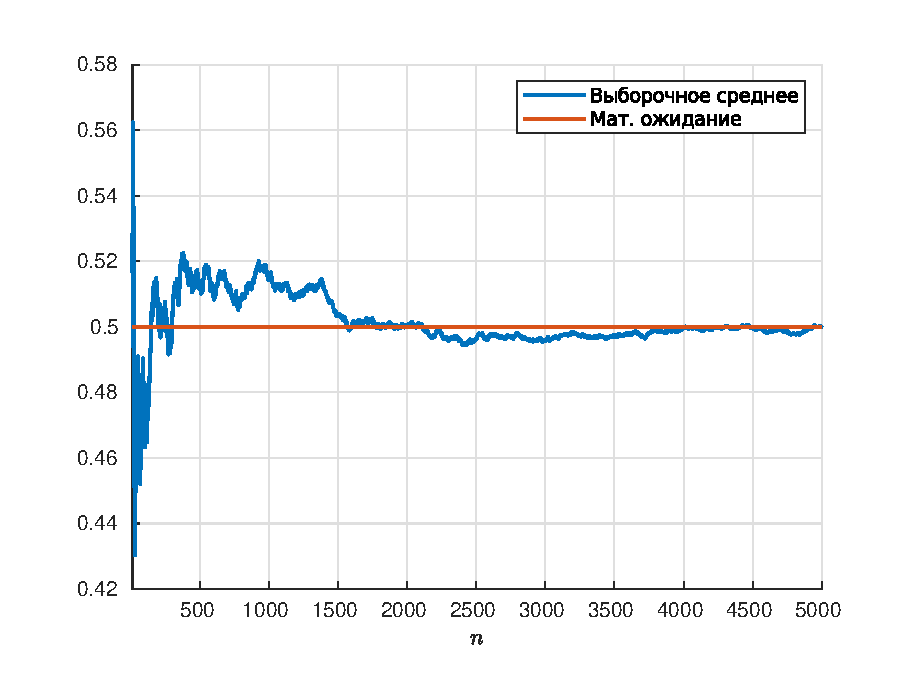
\includegraphics[width=\linewidth]{task_02/expectes10-5000.eps}
        \caption{Эмпирическое значение математического ожидания <<канторовой>> случайной величины~$X$.}
\end{figure}
\begin{figure}[t]
        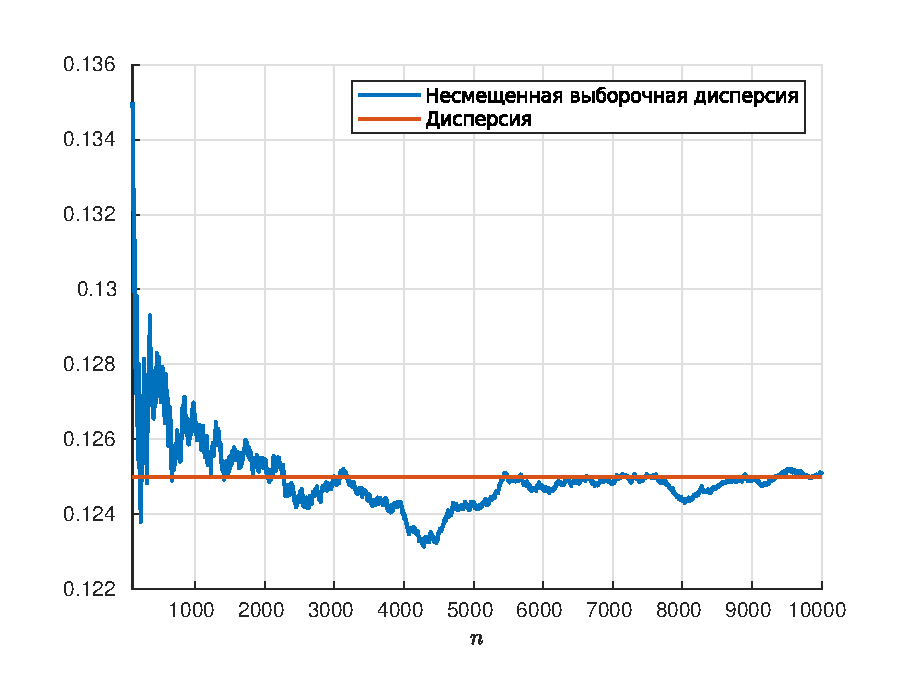
\includegraphics[width=\linewidth]{task_02/var100-10000.eps}
        \caption{Несмещенная выборочная дисперсия и теоретическая дисперсия <<канторовой>> случайной величины~$X$.}
\end{figure}
